\acresetall


%We will soon embark on a new era of discovery.
%A machine which can observe the universe in a whole new way is about to be
%turned on.
%The significance of this cannot be understated.
%We are about to make history.

%Of course, a drammatic introduction wouldn't be complete without a statement
%on how sentient beings have always gazed at the heavens in wonder.
%We still strive for this understanding and must never let it end.
%The struggles of humankind are too great to let our inspirations fizzle.
%Hope for the future is what sustains us.
%
%Something about Gallileo, Newton, Michelson, Einstein...

The physics community has been building gravitational wave detectors for
decades.
The resonant bar detectors of the past have given way to the new
interferometric detectors which have achieved impressive sensitivities.
These detectors are soon to be dramatically surpassed
by detectors with a more sophisticated optical layout, adding
signal recycling to the configuration.

This new generation of gravitational wave detectors are rapidly coming
online.
Advanced LIGO will be at design sensitivity within a year.
These new detectors will see further, by an order of magnitude over
initial LIGO, this corresponds to a 1000 times greater surveilled volume.
%A thousand times more detector volume.
At this sensitivity, one day of Advanced LIGO observations will survey a
larger space-time volume than the 2 years of observations with initial LIGO.
%And with the advancements in lock acquisition, we will surpass the entire
%integrated volume of initial LIGO in the blink of an eye.
aLIGO isn't a simple upgrade, it's literally a new detector.
Every component has been ripped out and replaced.
The laser source is new, pumping out a massive
%1.21 jigaWatts
180 Watts of power.
The radiation pressure noise associated with this power will start to
dominate the displacement noise of the new 40kg test masses.
%it will start to dominate even the new 40kg test masses.
From the state of the art coatings technology to the silicate bonded
monolithic fused silica fiber assemblies we have left virtually
%\footnote{with the interesting exception of the output mode cleaner, which
%serves as the readout point for the gravitational wave signal.}
nothing untouched.

As I am writing this,
the detector in Livingston is already beginning to surpass the
best sensitivity we ever had in initial LIGO. The detector at Hanford will
soon be sealed in it's capsule to embark on a journey into the farthest
reaches of the
universe\footnote{Manufacturing errors in the test mass coatings required a new
set to be installed, delaying the closure of the vacuum system.}.

Reflecting over my time at Syracuse, we have seen the Large Hadron Collider
turn on and confirm the existence of those things we were looking
for\footnote{the Higgs Boson}.
Of course I can't just leave the Higgs Boson as a footnote.
This is what gives matter its mass and as far as we know we can't have
gravitational waves without mass.
Well, we wouldn't exist without mass either, but that's beside the point...

%My time at Syracuse has brought me great joy.
%I have worked with many from throughout LIGO.

%Of course, my greatest joy comes from my family.
%Without them, I'm not sure I would have ever left my office/lab.
%We have had such a great experience here and made many friends of which we
%will never forget.


%For my children, it is your future that I live for.
%May your own inspirations come with great strength.

From this we begin,
\begin{equation}
F = ma\,.
\end{equation}


\section{Gravitational Waves}

The foundation of Einstein's theory of general relativity is that a freely
falling body's motion is governed by the local space-time curvature.
This curvature is in turn influenced by the presence of
matter\footnote{matter being stuff that has mass}.
This matter not only curves the space it occupies, but also curves the space
around it in such a way as to result in an acceleration on an object given by,
\begin{equation}
a = \frac{GM}{r^2} \;.
\end{equation}

Clearly, as matter moves through space, the curvature of space is changing.
Not only is the curvature changing is in the space in which the 
Having established that information cannot travel faster than the speed of light
the 'information' about how space must curve will be delayed.
From the multipole expansion of the mass distribution, the monopole (which is
the first term) is a scalar quantity that is simply the total
mass of the object.
The second term is, called the 'dipole' is a vector which is the sum of all the
bits of mass multiplied by their position vector from a fixed reference point.
The dipole term is identically the center of mass location times the total mass.
This term can change with time, however the first derivative $mv$ (momentum)
is conserved.
The third term is known as the quadrupole term.
It is this term which has a non zero second derivative that gives rise to a
wave equation.
The amplitude of the gravitational wave is,
\begin{equation}
h = \frac{2G}{c^4r}\ddot I \;.
\end{equation}
where the unitless term $h$ is the gravitational wave strain.
This strain is the $\frac{\Delta L}{L}$ perturbation on the background
space-time metric that WE are looking for.
Gravitational waves, being quadrupolar in nature, stretch space-time in one
direction while squeezing it in the orthogonal direction.

We look for the strain perturbations by measuring the distance between two
objects we call test masses.
In the simple case of a two test mass detector (one arm of LIGO) we are only
sensitive to half of the amplitude $h$ (assuming optimal orientation).
The simultaneous stretching and squeezing makes a differential length detector
a natural choice and with two orthogonal arms we are sensitive to the full
amplitude of the wave.
It is important to note that this factor of 2 increase in the signal, though
helpful, is not the primary motivation for two arms. 
The big benefit comes from common noise cancellation.
We can cancel out common length noise in the two arms because the gravitational
wave will couple directly into the differential degree of freedom in the
detector. See figure \ref{fig:ligoschematic}.


\begin{figure}
\tikzsetnextfilename{ligoschematic}
\centering
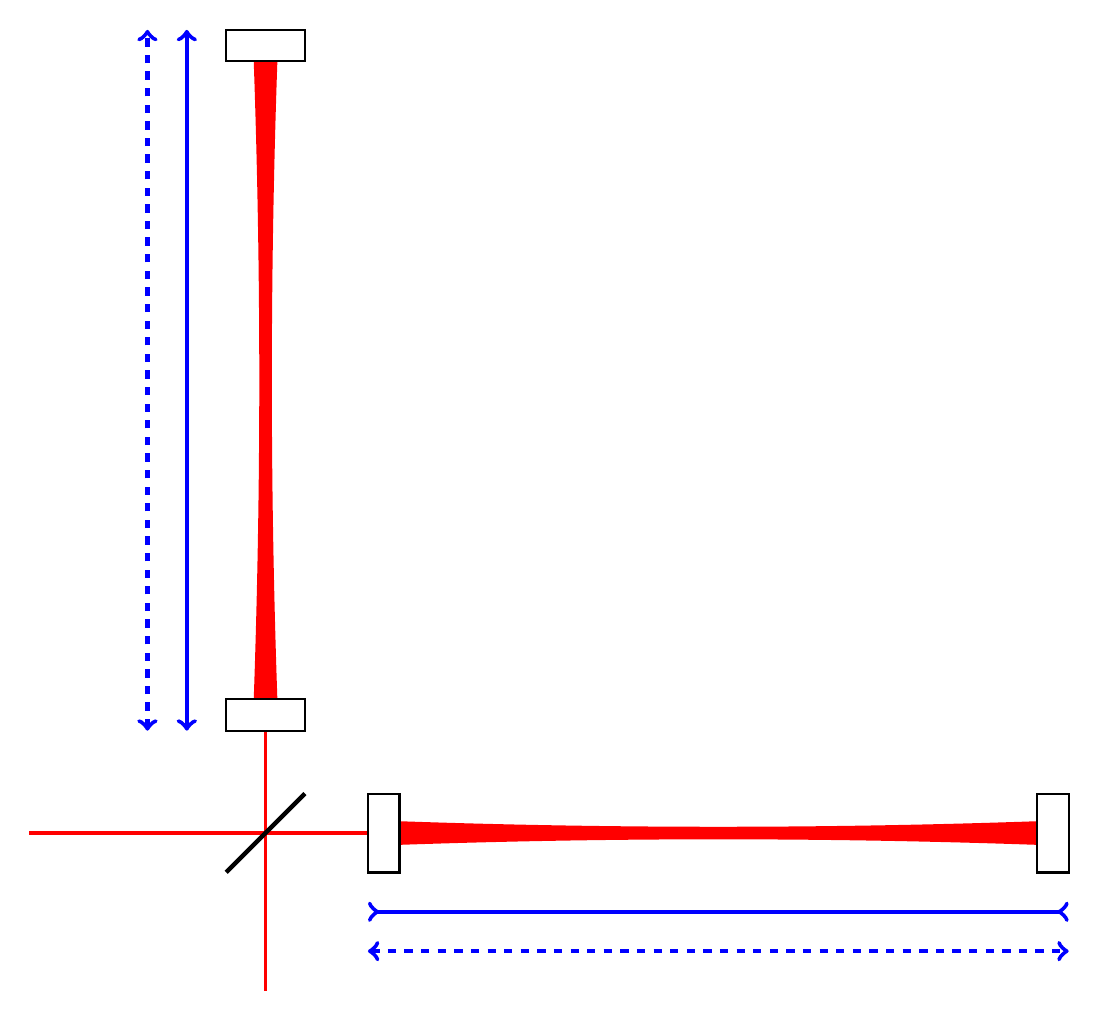
\begin{tikzpicture}
%  \draw[thick,rotate=45] (-1,-0.2) rectangle (1,0.2);
  \draw[very thick,red] (-3,0) -- (1.3,0);
  \draw[very thick,red] (0,0) -- (0,1.3);
  \draw[very thick,red] (0,0) -- (0,-2);
  \fill[red] (1.7,-0.15) arc (92:88:116.048) -- ++(0,0.3) arc (272:268:116.048) -- cycle;
  \fill[red] (-0.15,1.7) arc (-2:2:116.048) -- ++(0.3,0) arc (178:182:116.048) -- cycle;
  \draw[ultra thick] (-0.5,-0.5) -- (0.5,0.5);
  \draw[thick] (1.3,-0.5) rectangle (1.7,0.5);
  \draw[thick] (9.8,-0.5) rectangle (10.2,0.5);
  \draw[thick] (-0.5,1.3) rectangle (0.5,1.7);
  \draw[thick] (-0.5,9.8) rectangle (0.5,10.2);
  \draw[ultra thick,blue,<->] (-1,1.3) -- (-1,10.2);
  \draw[ultra thick,dashed,blue,<->] (-1.5,1.3) -- (-1.5,10.2);
  \draw[ultra thick,blue,>-<] (1.3,-1) -- (10.2,-1);
  \draw[ultra thick,dashed,blue,<->] (1.3,-1.5) -- (10.2,-1.5);
\end{tikzpicture}
\caption[LIGO Schematic]{This schematic shows the layout of a basic
    interferometric gravitational wave detector.
    Each arm of the interferometer is a Fabry-Perot cavity which circulates
    the light in the arms, increasing the response of the detector.
    The blue lines indicate the common (dashed) and differential (solid)
    degrees of freedom.
    The Michelson naturally reads out the differential degree of freedom which
    is free of common noise such as the intensity and frequency noise of the
    laser.
    }
\label{fig:ligoschematic}
\end{figure}

%A pea sized amount of neutron star material has the mass of about 100,000
%locomotives.

\section{Angular Control Using Optical Traps}

In Advanced LIGO we use an active feedback control for angular alignment of
the main mirrors.
We are limited in this setup by sensing noise.
By using optical traps we can bypass this limitation.

The sensing is done with a technique called wavefront sensing.
It is basically a \ac{pdh} lock with quadrant photo-diodes measuring
the differential \ac{pdh} signal from opposite quadrants of the photo-diode.

